%%%%%%%%%%%%%%%%%%%%%%%%%%%%%%%%%%%%%%%%%%%%%%%%%%%%%%%%%%%%%%%%%%%%%%%%%%%%%%%%%%%%%%%%%%%%%%%%%%%%%%
%
%   Filename    : chapter_1.tex 
%
%   Description : This file will contain your Research Description.
%                 
%%%%%%%%%%%%%%%%%%%%%%%%%%%%%%%%%%%%%%%%%%%%%%%%%%%%%%%%%%%%%%%%%%%%%%%%%%%%%%%%%%%%%%%%%%%%%%%%%%%%%%




\chapter{Research Description}
\label{sec:researchdesc}




This chapter is an overview of the research undertaken in the field of community detection in social networks. 
This chapter is divided into five sections which are the current state of the technology, research objectives, scope and limitations, significance of the research, and the research methodology.




\section{Overview of the Current State of Technology}
\label{sec:overview}


Social media has become much more prevalent in recent years. People can now participate in what is called microblogging, a way for people to share their thoughts, status, and opinions in short posts, like Twitter, where posts are limited to one-hundred and forty characters \cite{Java:2007}. As such, these social media platforms are a prime opportunity to mine sentiments and to detect communities in the social network. Social media can also be used to build user networks through users following other users, for example, in Twitter, creating a network of accounts.




Community detection is clustering multiple users into groups where users within the group are more similar than users from outside the group \cite{Tang:2010}. Community detection is necessary because it observes the interaction of multiple users in relation to specific similarity parameters such as followed users, post topics, and mentioned users. Numerous studies on community detection have already been done. 


\citeA{Zhang:2012} defined features such as text content similarity, URL similarity, hashtag similarity, following similarity, and retweeting similarity that can be used to identify similarity between two nodes and aggregated these similarities to detect communities. Their software provided the listings of users in each community. The following figure is a comparison of the method used by Zhang against random clustering.


\begin{figure} [h]
	\centering
	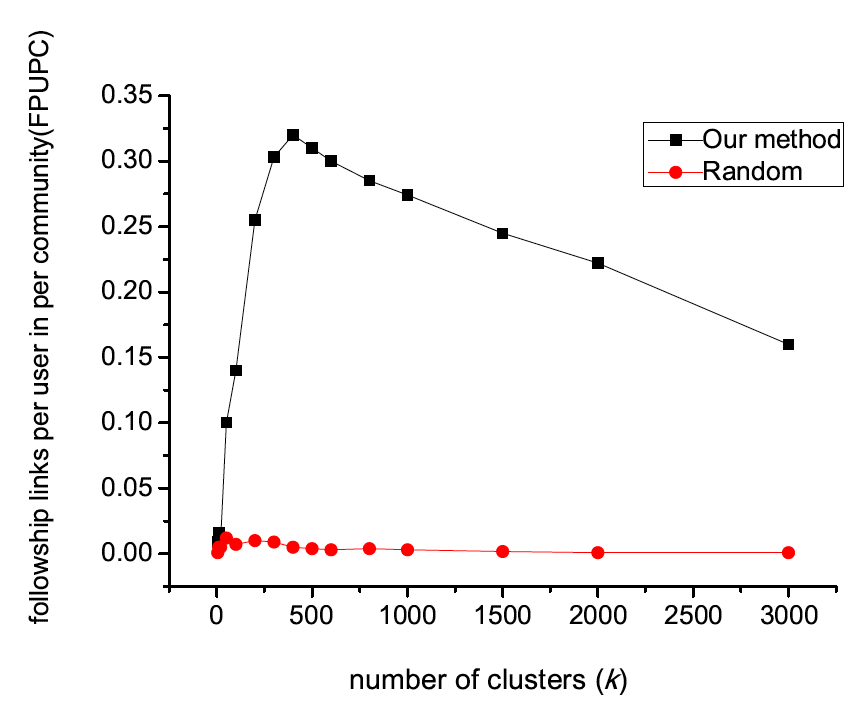
\includegraphics[width=0.5\textwidth]{Chapter1_Zhang}
	\caption{Results of Zhang’s community detection method compared to random clustering}	
\end{figure}



\citeA{Lim:2012:1} performed an inverted version in which they first defined interests and based on these interests, sought to extract communities from the network by identifying users that follow the top six celebrities, users with more than 10,000 followers, relating to the given interest. Their software generated the size and clustering coefficient of each community. The following figure shows the total number of communities formed by using certain algorithms such as the Clique Percolation Method and Infomap, which will be discussed in the review of related literature.



\begin{figure} [h]
	\centering
	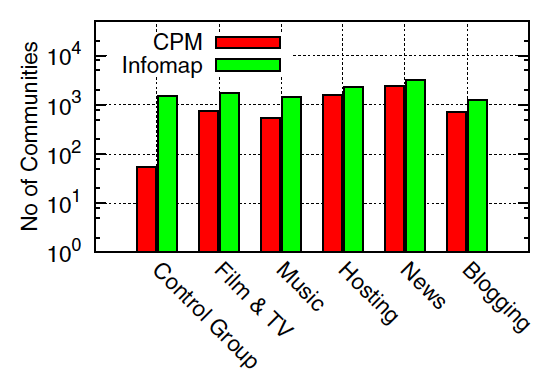
\includegraphics[width=0.5\textwidth]{Chapter1_Lim}
	\caption{Total number of communities formed using the Clique Percolation Method and the Infomap algorithm in the study done by Lim}	
\end{figure}

Individual opinions of a specific user towards another were also studied by \citeA{West:2014} combining sentiment analysis, using an L2-regularized logistic-regression classifier, with network analysis, inferring one user\vtick s opinion of another by analyzing their common links with other users. Their output was the area under the curve of the receiver operating characteristic (AUC/ROC) and the precision-recall curves (AUC/negPR). \par

In addition to these works, some visualizations have already been created such as SocialHelix by \citeA{Cao:2015}, which uses the temporal extent of social communities, topics or events discussed, and user responses to topics and events to classify users into two sides of the argument. They then depict the two sides of an argument as strands in a double helix and their intersections defines events.


\begin{figure} [h]
	\centering
	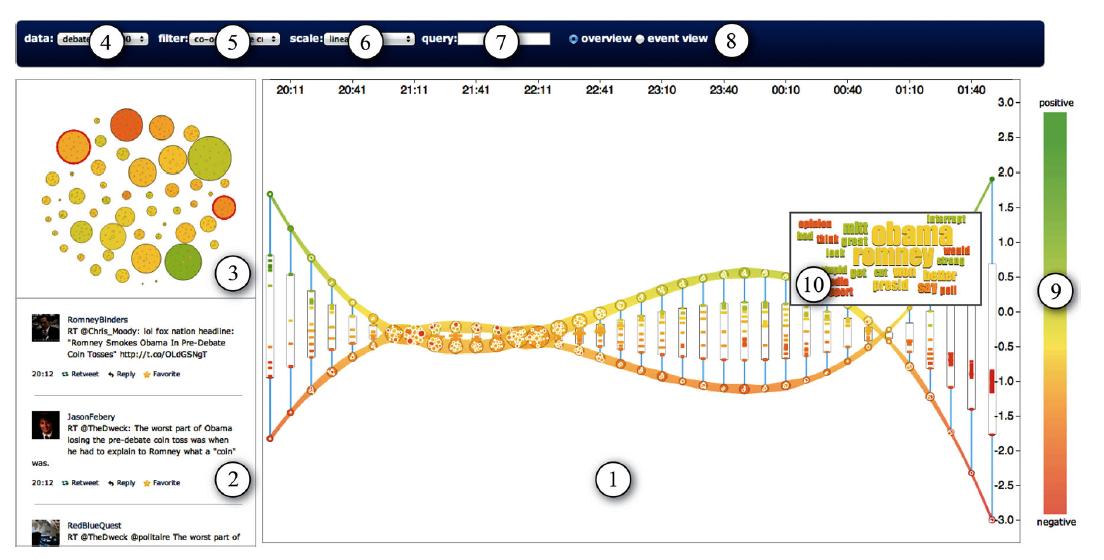
\includegraphics[width=0.5\textwidth]{Chapter1_Cao}
	\caption{Representation through SocialHelix of Twitter discussion surrounding the October 2012 U.S. presidential debate}	
\end{figure}



However, most of these studies already had preselected features and algorithms to work with or had specific features in mind before implementing their models. It would be interesting to compare the quality of communities produced by different combinations of algorithms and similarity parameters.


\section{Research Objectives}
\label{sec:researchobjectives}




\subsection{General Objective}
\label{sec:generalobjective}




To design and implement a tool that will detect communities based on varied combinations of detection algorithms and similarity measures.




\subsection{Specific Objectives}
\label{sec:specificobjectives}




\begin{enumerate}
	\item To build a corpus of social media data;
	\item To survey the various techniques and algorithms in detecting communities;
	\item To review the parameters/features to be used in detecting the communities;
	\item To survey evaluation metrics for the detected communities.
\end{enumerate}




\section{Scope and Limitations of the Research}
\label{sec:scopelimitations}




In order to perform a study on community detection, it is necessary to build a corpus of social media data. This research will cover searching for Application Programming Interfaces (API) that will allow extraction of data from Twitter and then using these APIs to build a body of data where community detection can be performed on. Data will include posts, profile information, and network information such as following list, follower list, and group membership.




Different techniques have been used in community detection. This research will consider algorithms used in other community detection works, including the fast greedy optimization of modularity, k-means clustering, and divisive or agglomerative hierarchical clustering.




Before the selected algorithms are implemented, it is necessary to identify which parameters/features/attributes indicate one user\vtick s similarity to another. Inquiry will be done to identify these parameters, specifically how to extract them based on the raw data. The research will be limited to sentiment analysis and elements which can be extracted from a user\vtick s post, which may include follow networks, hashtags, mentions, and retweets, which were mostly inspired from literature which focused on Twitter \cite{Deitrick:2013,Zhang:2012,Lim:2012:1}. 




After community detection, it is necessary to determine whether the detected communities are sensible. Inquiry will be done to find appropriate metrics in determining the accuracy of detected communities. These algorithms will include average mutual following links per user per community or FPUPC \cite{Zhang:2012}, modularity \cite{Deitrick:2013}.


\section{Significance of the Research}
\label{sec:significance}




Community detection is already a widely researched topic in the field of computer science. This study will contribute to that field by performing a comparative analysis of combinations of algorithms and parameters. The goal of this research is to compare and analyze how different combinations of these algorithms and parameters affect the communities generated, and use this information to improve the overall results of existing community detection algorithms. 


The results of the community detection algorithms are dependent on various similarity parameters that serve to reflect the real-life interactions and relations between users of a social network. Being able to generate improve the results of community detection algorithms will in turn allow the generation of more accurate, more true-to-life models of user relations. This information can be a very useful tool in the domains of online marketing and political analysis. Companies that are monitoring the performance of certain products or brands can use the results of these algorithms to improve their sales and marketing, by identifying which groups of people their product is strong with, and which groups of people it performs poorly with. Political analysts can monitor public reception of certain candidates in the same way.




\section{Research Methodology}
This chapter details the research activities to be done for the duration of this thesis. Our study will be in three main parts: the preparation phase, the iterative experimentation phase, and the analysis and finalization phase.




\subsection{Preparation}




This phase constituted the gathering of information pertinent to the study. This included reviewing related literature and building a theoretical framework. The theoretical framework step overlapped with the review of related literature step. This step included gathering implementation details for the variables in the experimentation phase: community detection algorithms found in the review of related literature; computing similarity parameters, including sentiment analysis and features in Twitter; and evaluation metrics. 




This phase included finding the necessary API\vtick s to use in collecting data from Twitter. Selection of the platform to host the data and a programming language to implement the model was also part of this phase\vtick s activities. 




It was necessary because it provided the theoretical framework around which the entire study will be based on, as well as deciding the platform and programming language to be used throughout the study. All design and implementation performed in the project was based on the information gathered in this phase.




\subsection{Iterative Experimentation}




This phase deals with design, implementation, and testing of multiple community detection models. Each iteration would differ based on two variables: a different similarity parameter and a different community detection algorithm. Each iteration will take two to three weeks to perform, depending on how many of the aforementioned variables differ and how different the given variable\vtick s implementation details are from the previous iteration\vtick s.




\subsubsection{Similarity Parameter Selection}




Since this study aims to produce an accurate visualization of communities in social media, it is necessary to find out which parameter would produce the best communities based on the evaluation metric found in the preparation phase. This is the reason why there will be multiple iterations. 




Based on the RRL and the Theoretical Framework, a similarity parameter will be selected from the features identified in the preparation phase.




\subsubsection{Community Detection Algorithm Selection}




In producing the visualizations of communities, it is also necessary to select the best community detection algorithm for the data, which is determined by using the evaluation metric on the produced communities. Each iteration would then deal with a different combination of similarity parameter and community detection algorithm.




Based on the RRL and the Theoretical Framework, a community detection algorithm will be selected. This algorithm must be compatible with the selected similarity parameter.




\subsubsection{Data Collection}




User data will be collected from Twitter. The API\vtick s will be used to gather the data. This will be done in order to have a corpus of data to perform the algorithms on. Afterwards, each user will be anonymized. This includes the username and the real name.  This anonymization is done to preserve the terms and conditions of using public data extracted from social media. 




Any other data transformation necessary for the parameter or the algorithm will then be performed.




\subsubsection{Model Design}




A model will be designed for the selected algorithm and similarity parameters. For the first iteration, this step should also include designing the model for the evaluation module i.e., the module which will evaluate the detected communities. This is done to organize the given algorithm and feature in a model that is ready for implementation.




\subsubsection{Model Implementation}




The majority of the iteration will involve implementing the given model in the language. For the first iteration, this step should also include the implementation of the evaluation metrics. This is done in order to have a working model that can be run on the collected data and tested for accuracy. Note that the evaluation metrics, specifically modularity, may be run as part of the algorithm to determine a stopping condition for the algorithm’s iteration.




\subsubsection{Model Evaluation}




The model will be run on the collected data for Twitter and the evaluation module will be run on the detected communities in order to measure the communities\vtick accuracy. This is done in order to evaluate how the selected parameter and algorithm performs on the collected data, which will be comparable at the end of the study to the results from other iterations, allowing the proponents to select which parameter-algorithm pair produces the most accurate communities in which particular social network.




\subsubsection{Documentation}




The documentation of the iteration will be finalized. Note that documentation should have been done regularly throughout the iteration, but this step is to ensure the quality and correctness of the documentation. This step will also include a retrospective on what worked in the previous iteration, what did not work, and how the development process can be improved. This step is done in order to ensure integrity in the data and documentation as well as to constantly improve the development process during the duration of the study.




\subsection{Analysis and Finalization}




This phase will involve revisiting the data collected from the multiple iterations and selecting which combination of parameters and algorithm resulted in the most accurate communities. This phase may include supplementary research in an attempt to see why some combinations produced better communities than others to have a more thorough understanding of the results. Finally, the proponents will produce a visualization using the best parameter-algorithm combination, satisfying the objective of the study. This step is necessary in order for the information gathered in this study to be presentable and to have a tangible output based on the results of the study.




\newpage
\begin{landscape}
	
	\section{Calendar of Activities}
	
	Table \ref{tab:timetableactivities} shows a Gantt chart of the activities.  Each bullet represents approximately
	one week worth of activity.
	
	%
	%  the following commands will be used for filling up the bullets in the Gantt chart
	%
	\newcommand{\weekone}{\textbullet}
	\newcommand{\weektwo}{\textbullet \textbullet}
	\newcommand{\weekthree}{\textbullet \textbullet \textbullet}
	\newcommand{\weekfour}{\textbullet \textbullet \textbullet \textbullet}
	
	\begin{table}[ht]   %t means place on top, replace with b if you want to place at the bottom
		\centering
		\caption{Timetable of Activities} \vspace{0.25em}
		\begin{longtabu} to 1.5\textwidth{|c|c|c|c|c|c|c|c|c|c|c|c|c|c|c|} \hline
			\centering Activities (2016-2017) & Jul & Aug & Sept & Oct & Nov & Dec & Jan & Feb & Mar & Apr & May & Jun & Jul & Aug \\ \hline
			Preparation (RRL) & \_\weekthree & \weekthree\_ &  &  & & & & & & &  &  & \_\_\weektwo & \weekone\_\_\_ \\ \hline
			Preparation (TF) & \_\weekthree & \weekthree\_ & \_\_\weektwo & & & &  &  & & & & & & \\ \hline
			Iterative Experimentation & & & & \weekfour & \weekfour & \weektwo\_\_ & \_\weekthree & \weekfour & \weekfour   & \weekfour & \weekfour & \weekfour & \weektwo\_\_ & \\ \hline
			Analysis and Finalization & & & & & & & & & & & & & \_\_\weektwo & \weekone\_\_\_ \\ \hline
		\end{longtabu}
		\label{tab:timetableactivities}
	\end{table}
\end{landscape}
